\documentclass[10pt]{article}

\usepackage[margin=1in, letterpaper]{geometry}
\usepackage{parskip}

\usepackage{amsthm, amsmath, amssymb}
\usepackage{gensymb}  % For use of degree symbol
\usepackage[pdftex]{graphicx}
\usepackage{hyperref}

\usepackage{enumerate} % For use of (a), (b), et cetera
\usepackage{booktabs}
\usepackage[margin=10pt, labelfont=bf, labelsep=period,
justification=justified]{caption}


% The following metadata will show up in the PDF properties
\hypersetup{
	colorlinks = true,
	urlcolor = black,
	pdfauthor = {Aaron Tran},
	pdfkeywords = {berkeley},
	pdftitle = {Astro 121, UG Radio Lab, Lab 3 - \today},
%	pdfsubject = {},
	pdfpagemode = UseNone
}

% Don't indent paragraphs
\setlength\parindent{0em}

% ===============
% Useful commands
% ===============
\newcommand {\mt}{\mathrm}
\newcommand {\unit}[1]{\; \mt{#1}}
\newcommand {\ints}{\mathbb{Z}}
% http://vemod.net/typesetting-units-in-latex

% ==========================
% Document specific commands
% ==========================

\begin{document}

% =======
% Titling
% =======
\begin{center}
\Large{Interferometer fringe measurements of Sun, Moon, and SRC at 11 GHz}

\large
Aaron Tran \\
\today \\
Leonardo Sattler Cassara, Ryan (Xin Xing) Gao, Patrick Kantorski, Salman Kahn
(PLSAR Collaboration) \\
Prof. Aaron Parsons, GSI Karto Keating, UGSI Baylee Bordwell
\end{center}
% ========
% Abstract
% ========
\section*{Abstract}


% ============
% Introduction
% ============
\section{Introduction}

Motivation -- measure source declinations and sun moon angular diameters
Pedagogical -- understand interferometry
Least squares fitting to back out meaningful astronomical numbers

% =======
% Methods
% =======

\section{Methods}

\subsection{Rotation matrices and ephemerides}

\subsection{Target selection and ephemeris plots}

\subsection{Interferometer design}

We made observations with a two-element multiplying interferometer.
The interferometer consists of two antennae (diameter $d = ? \unit{m}$) with
east-west baseline $b = 10 \unit{m}$ on Wurster Hall's roof
($37\degree 52' 12.7'' \unit{N}$, $-122\degree 15' 15.8'' \unit{E}$).

Beam size, accuracy, parameters.

\subsection{Observing campaign}

Days, times, targets.  Ephemeris plots go here
Give table.

Interferometer pointing and rehoming.
% =======
% Results
% =======
\section{Results}

\subsection{Declination measurement from fringe frequencies}

\begin{figure}[!ht]
    \centering
    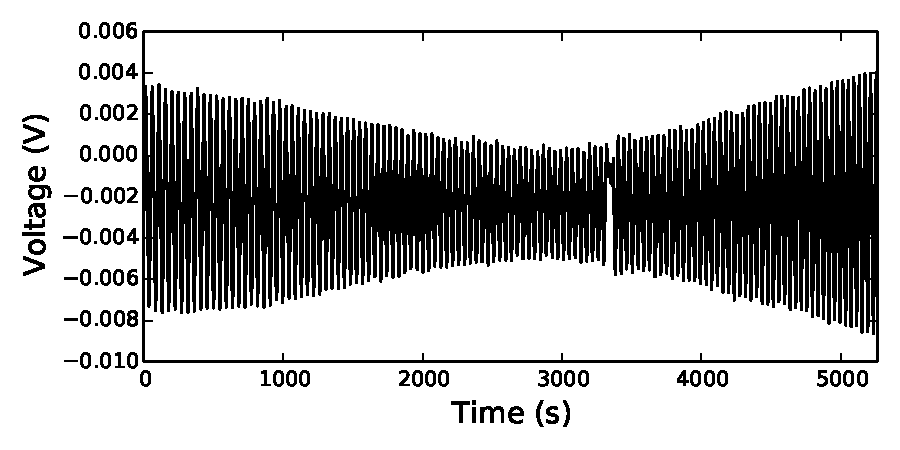
\includegraphics[scale=1]{code_analysis/sun_test.pdf} \\
    \caption{Shitty caption}
\end{figure}

\subsection{Angular diameters of the Sun, Moon}

% ==========
% Discussion
% ==========
\section{Discussion}

% ===========
% Conclusions
% ===========
\section{Conclusions}



\section{Acknowledgments}

Much props to Karto for his dedication in getting the interferometer back up
and running, and to Baylee/Karto both for porting IDL stuff.

\section{Electronic supplement}

All supporting files are stored on the repository:\\
\href{https://github.com/aarontran/ay121}
{https://github.com/aarontran/ay121/lab3/}.

\end{document}
